\chapter{\glsentrylongsp{ci}}
\label{ch:sota-ci}

\begin{marginfigure}
	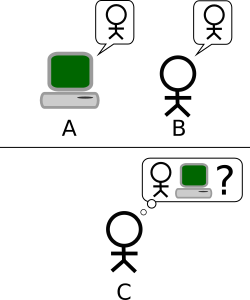
\includegraphics{turing-test}
	\caption{Ilustración del Test de Turing. Propuesto modelo para probar si una máquina es capaz de exhibir comportamiento inteligente similar al del ser humano. Hay tres participantes, dos humanos ($A$ y $C$) y una máquina ($B$), separados entre sí pero pudiendo intercambiarse mensajes de texto. $C$ envía preguntas a $A$ y $B$ sin saber quién es humano y quién es máquina y éstos le responden. Si $C$ no es capaz de identificar qué participante es la máquina, se puede concluir que la máquina es inteligente. Fuente: Hugo Férée, via Wikimedia Commons.}
	\label{fig:turing-test}
\end{marginfigure}

El comportamiento de una persona se ve influenciado por una infinidad de variables. Identificar las relaciones entre éstas es en la mayoría de las ocasiones una tarea que va de lo muy difícil a lo imposible, más aún si añadimos que éstas son muy numerosas y pueden llegar a ser imposibles de cuantificar o incluso de detectar.

La \ac{ci} engloba un conjunto de técnicas que facilitan enormemente estas tareas. En este capítulo se ofrece una perspectiva de la literatura actual sobre las técnicas de la \gls{ci} que son de interés para esta tesis. Introduciremos el concepto y las nociones de \enquote{agente} y de \enquote{aprendizaje} para posteriormente introducir algnuas de las técnicas utilizadas dentro del área. Por último, desarrollaremos las tres técnicas principales sobre las que reposa el trabajo teórico de esta tesis: \glsentrylongplsp{ann}, \glsentrylongsp{fl} y \glsentrylongsp{cev}.

\section{\glsentrylongsp{ai} vs. \glsentrylongsp{ci}}

¿Qué es la \ac{ci}? Para entender el significado de éste término tenemos que entender cómo ha evolucionado el término \ac{ai} a lo largo de los años.

El primer concepto a introducir es el de \enquote{conexionismo}. Se puede considerar a Santiago Ramón y Cajal como principal precursor de esta idea por sus trabajos acerca de la estructura de las neuronas y de sus conexiónes (e.g. \cite{y1888estructura} y~\cite{ramon1904textura}). Otros prefieren citar los trabajos de McCulloch y Pitts sobre \ac{ann} (\cite{McCulloch1943}) o de Donald Hebb acerca de la teoría del aprendizaje(\cite{hebb19680}) como primeros trabajo sobre este tema. Independientemente de su origen, el conexionismo postula que la mente y el conocimiento surgen de redes formadas por unidades sencillas interconectadas (i.e. neuronas).

\begin{marginfigure}
	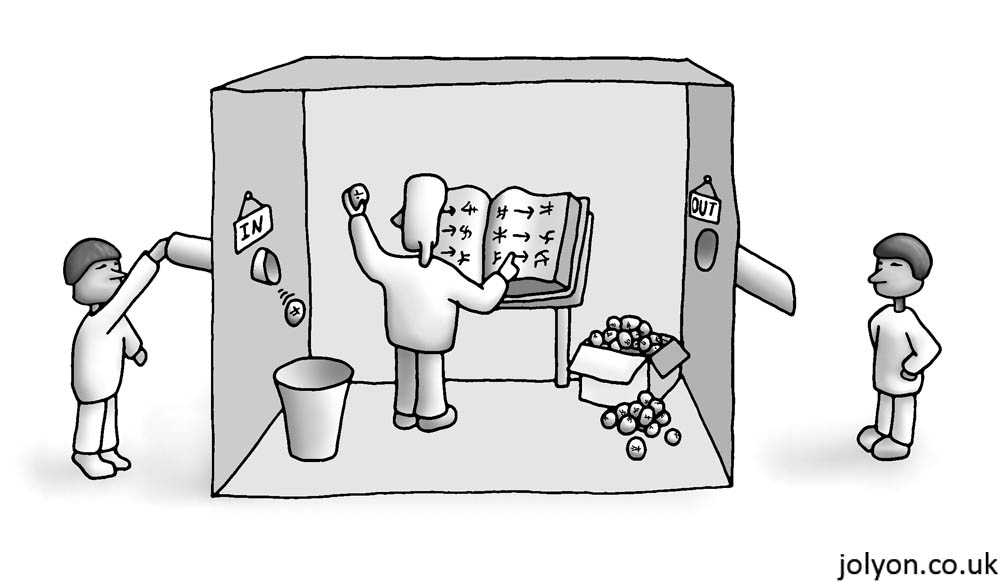
\includegraphics{chinese-room}
	\caption{El expermiento mental de la habitación china (ver~\cite{preston2002views}) propuesto por John Searle. Se trata de un Test de Turing donde la máquina ha aprendido a hablar chino y es reemplazada por una persona que no sabe nada del idioma pero que va equipada con manual de correspondencias del tipo \enquote{entra esta secuencia de ideogramas, sale esta secuencia de ideogramas}. Cuando una persona le manda mensajes en chino, esta otra responde, pero ¿podemos decir que dicha persona sabe chino? Evidentemente no. Entonces, cómo podemos asegurar que la máquina reemplazada ha \enquote{aprendido} chino. Autor: Jolyon Troscianko (http://www.jolyon.co.uk/)}
	\label{fig:chinese-room}
\end{marginfigure}

Por otro lado, en 1950, Alan Turing publicó un artículo que comenzaba con la frase \textit{\enquote{Can machines think\sidenote{El propio concepto de \enquote{pensar} es en sí un tema controvertido en el propio ser humano: ¿pensar es algo inherentemente biológico? ¿surge de la mente? Tanto si sí como si no, ¿de qué forma lo hace? Por ello existen detractores de la validez del Test de Turing. Por ejemplo, el experimento de la habitación china (figura~\ref{fig:chinese-room}) nace precisamente como refutación de dicho test, aunque puede llevar a cuestiones quizá más intrigantes. Por ejemplo, si la máquina es capaz de realizar una acción sin entender lo que hace y por qué lo hace, ¿qué garantías tenemos de que el humano sí es capaz? Si los ordenadores operan sobre símbolos sin comprender el verdadero contenido de éstos, ¿hasta qué punto los humanos lo hacen de forma diferente?.}?~\cite{turing1950computing}}}, introduciendo el famoso Test de Turing para determinar si una máquina es o no inteligente (figura~\ref{fig:turing-test}). Se puede considerar este momento como el punto donde se estableció el objetivo a largo plazo del campo de la \ac{ai}, ya que en el artículo Turing propuso un método para determinar si una máquina era capaz de exhibir comportamiento inteligente. Sin embargo, no fue hasta $1956$ en la Conferencia de Dartmouth~\cite{mccarthy1956dartmouth} donde John McCarthy acuñó el término~\ac{ai} a la vez que presentó el tema de la conferencia como la pregunta realizada por Turing en dicho artículo.

A partir de este punto la investigación en~\ac{ai} recibió muchísima atención por parte de investigadores y gobiernos, lo que se tradujo en financiación. Los estudios estaban dominados por aquellos relacionados con las idesa del conexionismo hasta que en $1969$, se publicó el libro \textit{Perceptrons}~\cite{minsky1969perceptrons} de Marvin Minsky y Seymour Papert, donde se expusieron las limitaciones de los modelos de \acp{ann} desarrollados hasta la fecha. El impacto fue tal que la investigación en \gls{ai} se abandonó casi por completo. Concretamente el conexionismo dejó de estar presente en la literatura científica durante dos décadas. Es lo que se conoce como \textit{AI Winter}\sidenote{Es injusto achacar el \textit{AI Winter} sólo al libro \textit{Perceptrons}. El \enquote{efecto gurú} del libro fue sólo la gota que colmó el vaso. A la emoción inicial por los avances le siguieron muchos años de promesas incumplidas, investigación sin resultados significativos, limitaciones de hardware, aumento de la complejidad del software (los comienzos de la crisis del software. Ver~\cite{dijkstra1972humble}). Todo ello provocó un desinterés y una disminución de la financiación que se retroalimentaron la una a la otra.}.

El interés por el campo volvió de nuevo a principios de $1980$ con la aparición en escena de los prmieros Sistemas Expertos (\cite{russell2003artificial}), los cuales se consideran como el primer caso de éxito en la \gls{ai}. A finales de la década, sin embargo, empezaron a resurgir los enfoques conexionistas, en gran parte por la aparición de nuevas técnicas de entrenamiento en perceptrones multicapa o por conceptos como activación no lineal en neuronas (e.g.~\cite{rumelhart1985learning} o~\cite{cybenko1989approximation}). En este momento los sistemas expertos empezaron a perder interés frente al nuevo avance del conexionismo\sidenote{A esta década se la conoce como segundo \textit{AI Winter} dado que la investigación sobre Sistemas Expertos disminuye. Sin embargo no fue un abandono tan acusado como el del primer \textit{AI Winter}.}.

Mientras que el enfoque clásico de la \ac{ai} postulaba que la mente operaba de la misma manera que una máquina de Turing, es decir, mediante operaciones sobre un lenguaje de símbolos, el enfoque del conexionismo postulaba que la mente, el comportamiento inteligente, emergía de modelos a más bajo nivel. Esto provocó que algunas voces se alzaran contra lo que se consideraba el \enquote{enfoque incorrecto} de la \ac{ai}. Sin embargo, otras técnicas alineadas con el conexionismo (debido a su enfoque de comportamiento emergente y aproximación como lo son la \ac{fl} o los \acp{ga}) ganaban popularidad y alimentaban el éxito cosechado por este \enquote{enfoque incorrecto}\footnote{Es comprensible ya que el método clásico produce modelos fáciles de interpretar mientras que el enfoque conexionista produce modelos cuyo funcionamiento en general no es del todo deducible. Sin embargo, existen problemas con alto grado de complejidad muy difíciles (o imposibles) de modelar. Más aún cuando éstos son de naturaleza estocástica~\cite{siddique2013computational}.}.

Esto provocó una explosión de terminologías para diferenciar las investigaciones de la propia~\ac{ai} clásica. Por un lado se evitaba el conflicto, nombrando lasáreas de trabajo con un término más acorde con el comportamiento o técnica utilizada. Por otro, se separaba de las connotaciones negativas que fue cosechando la \ac{ai} con el paso de los años, \enquote{promesas, pero no resultados}).

Lo verdaderamente interesante es ver la evolución de la literatura, y por tanto de los objetivos de la \ac{ai} durante estos años. En el nacimiento del campo, se buscan literalmente máquinas que piensen como humanos, o al menos seres racionales, con mente. Con el paso de los años (y los continuos choques contra la realidad), la literatura va tendiendo hacia la búsqueda de conductas y comportamientos inteligentes cada vez más específicos. Este hecho se hace más patente en este momento, donde cada investigación se nombra de cualquier forma menos con el término \ac{ai} (e.g \ac{ml}, \acp{rs}, o \ac{nlp}). Es evidente que la \ac{ai} se puede observar desde diferentes puntos de vista, todos perfectamente válidos. En~\cite{russell2003artificial}, tras un análisis de las definiciones existentes en la literatura por parte de diferentes autores, se hace énfasis en este hecho mostrando los diferentes puntos de vista a la hora de hablar de lo que es la \ac{ai}. El resumen se puede observar en la figura~\ref{fig:different-povs-ai}.

\begin{figure}
	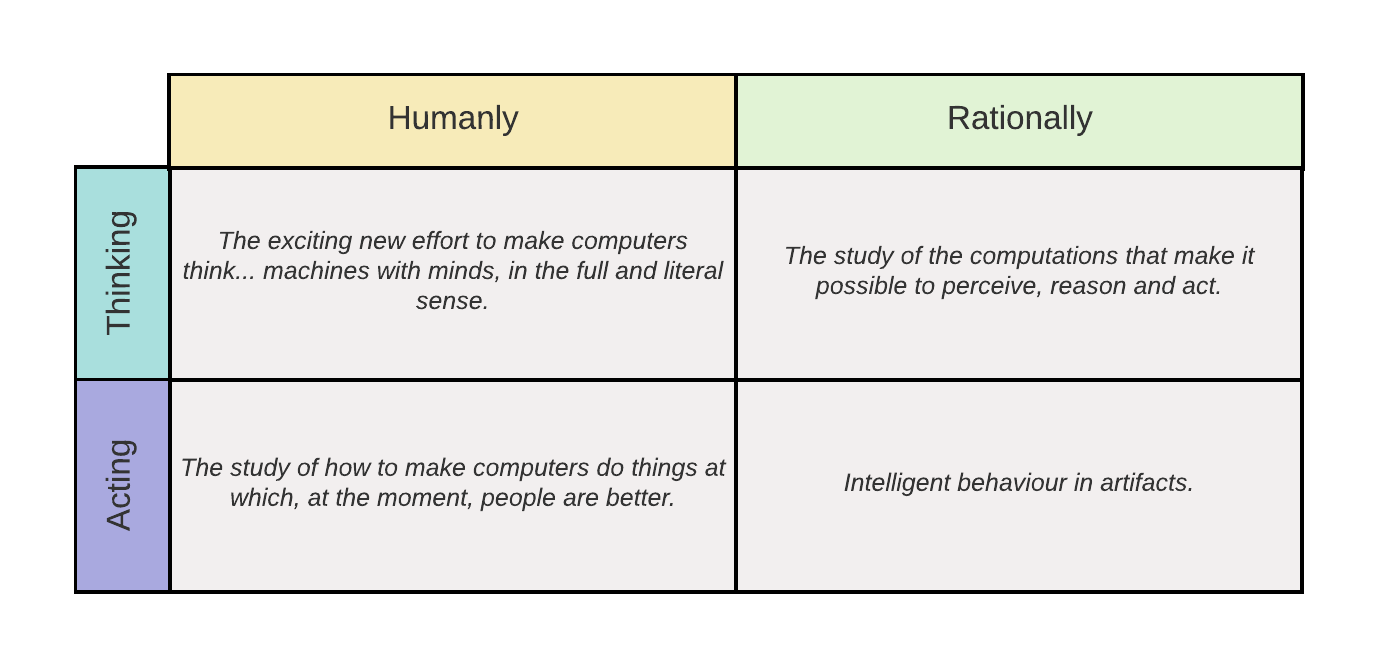
\includegraphics{different-povs-ai}
	\caption{Objetivos que persigue la~\glsentrylongsp{ai}. Las filas diferencian entre pensamiento o comportamiento mientras que las columnas separan entre inteligencia humana o inteligencia racional. Fuente: \textit{Artificial Intelligence: A Modern Approach ($3^{rd}$ Ed.)},~\cite{russell2003artificial}.}
	\label{fig:different-povs-ai}
\end{figure}

Volviendo al tema de la terminología, muchas de las diferentes técnicas se fueron agrupando dentro de diferentes áreas. Una de ellas es la conocida como \glsentrylong{ci}. Dado que persigue el mismo objetivo a largo plazo y que surje de la propia \ac{ai} parece lógico mantenerla como un subconjunto y no como un nuevo campo del conocimiento humano. Sin embargo, algunos autores abogan por que la \ac{ci} es un campo diferenciado de la \ac{ai}.

Podemos definir la \ac{ci} como la \enquote{\textit{rama de la \ac{ai} que aporta soluciones a \textbf{tareas específicas} de forma \textbf{inteligente} a partir del aprendizaje mediante el uso de \textbf{datos experimentales}}}. A diferencia de la aproximación clásica de la \ac{ai}, se buscan aproximaciones a las soluciones y no las soluciones exactas. Esto es debido a que muchos problemas son de naturaleza comlpeja, ya sea por la erlación entre sus multiplas variables, a la falta de información o a la imposibilidad de traducirlos a lenguaje binario.

Se puede fijar el año $1994$ como el que el término \ac{ci} nace como área, coincidiendo con el cambio de nombre del \textit{IEEE Neural Networks Council} a \textit{IEEE Computational Intelligence Society} (\url{http://cis.ieee.org/}). Poco antes, en $1993$, Bob Marks en su trabajo~\cite{bezdek1993intelligence} presentó las que él consideraba diferencias fundamentales entre la \ac{ai} y la \ac{ci} resumiéndolas en la siguiente frase.

\blockquote{Neural networks, genetic algorithms, fuzzy systems, evolutionary programming, and artificial life are the building blocks of CI.}

Durante estos años ganaba popularidad también el concepto del \ac{sc}. Éste engloba las técnicas que buscan resolver problemas con información incompleta o con ruido. Debido a que el conjunto de técnicas definidas como consituyentes del \ac{sc} son las mismas que las de la \ac{ci} algunos autores consideran ambos términos equivalentes. Nosotros consideramos que el \ac{sc} es un punto de vista de la computación más que de la \ac{ai} en contraposición con el \ac{hc}, y que la \ac{ci} hace uso de métodos del \ac{sc}\sidenote{El \ac{hc} es como se define la computación convencional frente al \ac{sc}. El \ac{hc} basa sus técnicas en aquellas basadas en modelos analíticos definidos de forma precisa y que en ocasiones requieren mucho tiempo de cómputo. Están basados en lógica binaria, análisis numérico, algoritmos y respuestas exactas. El \ac{sc} por otro lado es tolerante a la imprecisión y al ruido y tiende a llegar a soluciones aproximadas de manera más rápida. Se basa en modelos aproximados, emergencia de algoritmos y modelos estocásticos.}.

\section{Concepto de agente}

\section{Aprendizaje}

La resolución clásica a un problema suele ser la aplicación de una secuencia de instrucciones basadas en un conjunto de símbolos (e.g. una función escrita en el lenguaje de programación C). Esta forma de solucionar un problema no \textit{aprende} a solucionarlo. Se puede interpretar como que la solución está grabada en su memoria.

En la aproximación de la \ac{ci}, existen modelos y existen técnicas para hacer aprender esos modelos. La aplicación de dichas técnicas es lo que se conoce como \textbf{aprendizaje}. Las técnicas de aprendizaje en \ac{ci} se suelen clasificar en $2$ paradigmas:

\begin{itemize}
	\item \textbf{Supervisado}. El entorno presentado al modelo consiste en un conjunto de la forma $D = {(I_i, O_i) | \forall i \in \mathbb{N}}$, donde cada $O_i$ es la salida esperada del modelo a la entrada $I_i$. Los algoritmos tratarán de ajustar el modelo todo lo posible para que las salidas obtenidas sean lo más parecidas a las salidas originales. Este paradigma de entrenamiento suele estar relacionado con problemas de \textit{regresión}.
	\item \textbf{No supervisado}. Al modelo se le ofrece un conjunto de la forma $D = {I_i | \forall i \in \mathbb{N}}$, donde cada $I_i$ es una entrada al problema, pero del que no conocemos la salida. Los algoritmos dentro de esta categoría harán uso de estos datos para ir reajustando el modelo tratando de encontrar las estructuras ocultas entre dichos datos (e.g. patrones, correlaciones o clases). Es un paradigma de entrenamiento íntimamente relacionado con problemas de \textit{clasificación}.
\end{itemize}

Algunos autores hacen uso de técnicas pertenecientes a ambos paradigmas en forma de aproximación híbrida (\TODO buscar referencias) para \TODO{ver qué coño buscan con este tipo de aproximaciones. Creo que los auto-encoders en deep learning serían un buen ejemplo}.

Otros, añaden un paradigma más a estos dos existentes, el denominado aprendizaje \textbf{por refuerzo}. Sin embargo, nosotros preferimos considerarlo como un tiop de aprendizaje supervisado, ya que la única característica que lo diferencia es que es un tipo de aprendizaje que se usa en entornos de aprendizaje \textit{on line} ajustando el modelo en función de los estímulos percibidos del entorno por sus acciones sobre el mismo, y no en un entorno aislado previo de entrenamiento (\textit{off line}), como la práctica totalidad de técnicas supervisadas y no supervisadas.

\section{Ténicas en la \Glsentrylongsp{ci}}

¿Qué técnicas se usan actualmente y sobre qué problemas?

\section{\Glsentrylongplsp{ann}}

Una \acrlongsp{ann} puede considerarse como una herramienta que trata de replicar las funciones cerebrales de un ser vivo de una manera muy fundamental (esto es, desde sus componentes más básicos, las neuronas) basándose para ello en estudios de neurobiología y de ciencia cognitiva moderna del cerebro humano\sidenote{Aún apoyándose en la topología y funcionamiento del cerebro humano para realizar el símil, lo cierto es que dichos modelos distan aún de considerarse \textit{cerebros artificiales}. La red neuronal más compleja hasta la fecha es la propuesta en~\cite{TraskANDREWTRASK}, con alrededor de $160.000$ parámetros a ser ajustados (podemos abstraernos y pensar en ellos como conexiones entre neuronas). Como dato anecdótico, se estima que sólo en el neocórtex (ver figura~\ref{fig:neocortex}) del ser humano existen alrededor de $20.000$ millones de neuronas, cada una de las cuales conectada a entre $100$ y $100.000$ neuronas vecinas (\cite{Pakkenberg1997}). Esto supone entre $2 \cdot 10^{12}$ y $2 \cdot 10^{15}$ conexiones. Tecnológicamente hablando, la sensación esque estamos aún a años luz de aproximarnos siquiera a la complejiadd de un cerebro humano.}.

\begin{figure}
	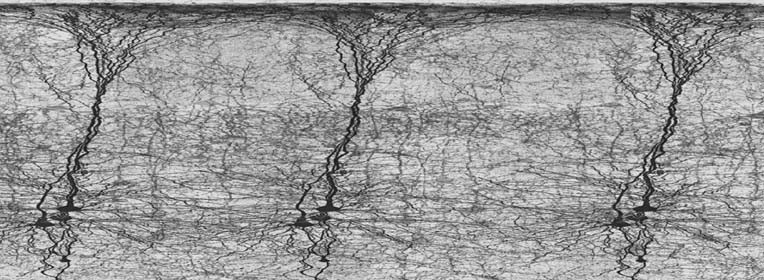
\includegraphics{neocortex}
	\caption{Una sección del neocórtex humano, región asociada a las capacidades cognitivas y que supone alrededor de un $76\%$ del volumen total del cerebro humano. Está distribuído en $6$ capas y miles de columnas que las atraviesan, cada una con alrededor de $10.000$ neuronas y un diámetro de $0.5mm$. Fuente: \textit{Blue Brain Project EPFL}, \url{http://bluebrain.epfl.ch/}.}
	\label{fig:neocortex}
\end{figure}

Se puede establecer el trabajo \enquote{A logical calculus of the ideas immanent in nervous activity} (\cite{McCulloch1943}) como el primero en esta disciplina y, aunque existen muchas y muy diferentes tipologías y formas de operar con redes, la conceptualización de su funcionamiento es la misma: unidades (i.e. neuronas) interconectados mediante enlaces por los que fluye la información de manera unidireccional, donde algunas de dichas unidades sirven de entrada al sistema (i.e. entradas o sensores), otras sirven de salida del sistema (i.e. salidas y actuadores) y otras como elementos internos (i.e. ocultas), y donde las conexiones se ajustan mediante un proceso denominado \textit{entrenamiento}.

Una \ac{ann} es independiente del modelo del problema a solucionar. Se la puede considerar como una caja negra que aprende las relaciones que subyacen en los datos del problema para abstraer el modelo a partir de éstas. Estas características de aprendizaje y abstracción son los factores determinantes por los que son usadas en prácticamente todas las áreas de la ciencia y de la ingeniería (\cite{Du2006}).

\subsection{Neurona artificial}

\subsection{Caracterízación y topologías}

\subsection{Aprendizaje en \glsentrylongplsp{ann}}

\section{\Glsentrylongsp{fl}}

La lógica matemática (y por extensión la teoría de conjuntos)\sidenote{Se puede establecer el siglo IV a.C. como el momento del nacimiento de la lógica dentro de la física Aristotélica, que permaneció inalterada hasta los trabajos de Galileo (cita?) y Newton (cita, seguramente el Principia Matematica) en el siglo XVI. d.C., momento en que se separó y permaneció como disciplina paralela perteneciente más al campo de la filosofía que de la física y la matemática. Empezó a relacionarse de nuevo con la matemática a principios del siglo XIX y a principios del siglo XX la lógica y la teoría de conjuntos pasaron a convertirse en partes indispensables la una de la otra. Por ello suelen ir de la mano cada vez que se habla de la una y de la otra. La evolución de la teoría de conjuntos (Cantor, finales del siglo XIX, buscar referencia) y su unión con la lógica es una época bastante convulsa dentro de la historia de la matemática pero esta tesis no es lugar para su desarrollo. Por ello se ofrece la referencia al libro \textit{La historia de la matemática} de Miguel de Guzmán (referencia. Poner la página. Lo mismo no es de aquí y es del libro de "Los lógicos", pero estoy casi seguro de que es aquí.) en caso de que el lector tenga interés en el tema.} tiene como misión servir de fundamento del razonamiento matemático. Se basa en la definición precisa y con rigor de un razonamiento evitando cualquier tipo de ambigiüedad y de contradicción. Es por ello que la lógica tradicional no suele servir como fundamento de razonamientos del mundo real.

Los conceptos que se manejan en el mundo real suelen ser vagos, llenos de imprecisiones. Además tienden a ser nombrados cualitativamente, no quantitativamente, y cuando existe una correspondencia, ésta suele estar marcada por la subjetividad de los términos.

Explicar lógica difusa y control difuso. Indicar los controladores difusos de segundo, tercer y sucesivos niveles.

\subsection{Teoría de conjuntos difusos}

A diferencia de los conjuntos tradicionales, los conjuntos difusos expresan el grado de pertenencia de un elemento a la categoría representada por el conjunto. La definición podría escribirse de la siguiente manera:

\TODO{Creo que habría que definir antes qué es un dominio}

\begin{definition}
	Sea $X$ una colección de elementos. Se define al \textbf{conjunto difuso} $F$ como un conjunto ordenado de pares de la forma $F = {(x, \mu_F(x)) | x \in X}$, siendo $\mu_F(x) \in [0, 1] \forall x \in X$.
	\label{def:fuzzy-set}
\end{definition}

La función de la definición~\ref{def:fuzzy-set} se denomina \textbf{función de pertenencia}, y caracteriza unívocamente a un conjunto difuso del dominio de $X$.

\TODO{Quizá aquí habría que decir qué es una partición de nu dominio}

\subsection{Operaciones entre conjuntos}

La unión, intersección y el complemento son operaciones básicas en la teoría de conjuntos. \TODO hablar aquí de tnorm, tconorm y complemento, pero someramente. No hay que enrollarse demasiado.

\subsection{Razonamiento}

En \cite{Ma} hay un capítulo de razonamiento que parece que está guay. Revisarlo un poco a fondo a ver si merece la pena tirar or ahí.

\subsection{Sistemas de inferencia difusa}

Los \acp{fis} o \acp{fcs} son sistemas que utilizan el razonamiento difuso para inferir una respuesta a partir de un conjunto de entradas. Habitualmente son divididos en tres bloques conceptuales, los cuales se ilustran en la figura XXX:

\begin{itemize}
	\item \textbf{Fuzzificación}. Traducir los valores de entrada en crudo del dominio sobre el que está definida cada variable lingüística a sus respectivos grados de pertenencia a conjuntos difusos a través de sus funciones de pertenencia. \TODO Ojo, algnuos controladores toman como valores de entrada conjuntos difusos según \cite{Ma}. Habrá que buscar sobre ello.
	\item \textbf{Inferencia}. Realiza todo el proceso de razonamiento difuso a partir del conjunto de reglas qeu dan significado a este controlador difuso.
	\item \textbf{Defuzzificación}. Traduce los conjunto difuso resultado del proceso de inferencia a valores del los dominios sobre los que están definidos dichos conjuntos difusos. \TODO En un sugeno, la salida es una función directamente así que se podría especificar que en un tipo Sugeno,se puede ver como que la salida son sólo singletones, manteniendo la generalización del proceso de funcionamiento de un \ac{fis}.
\end{itemize}

Hablar someramente de los tres tipos clásicos que se usan, e indicar que al final los más usados son el Mandamni y el Sugeno. Añadir también quizá una tabla comparativa enter los tres o al menos entre los dos principales:

El consecuente de un \ac{fis} de tipo Mandamni siempre es un conjunto difuso. Por tanto, el proceso de sacar un valor crisp es costoso. Lo bueno, se mantiene significado semántico de las salidas. El consecuente en un Sugeno es un valor, y se puede decir que no necesita proceso de defuzzificación. Si embargo, la respuesta pierde significado semántico si la suma de la fuerza de salida no es 1 (no entiendo qué quiero decir con esto).


\section{\Glsentrylongsp{cev}}

Explicar qué es la cev, la evolución de conceptos distintos a distintas escuelas de pensamiento del mismo concepto. 